\documentclass[runningheads]{llncs}

\usepackage{algorithm}
\usepackage{algpseudocode}
\usepackage{amsmath}
\usepackage{graphicx}
\usepackage{subcaption}
\captionsetup{compatibility=false}
\usepackage{multirow}
\usepackage{relsize}
\usepackage{booktabs}
\usepackage{tabularx}
\newcolumntype{R}{>{\raggedleft\arraybackslash}X}
\usepackage{tikz}
\usetikzlibrary{positioning}
\usetikzlibrary{calc}
\usetikzlibrary{backgrounds}
\usetikzlibrary{arrows.meta}
\tikzset{
    between/.style args={#1 and #2}{
    	at = ($(#1)!0.5!(#2)$)
    }
}

\setlength{\belowcaptionskip}{-1em}

\begin{document}

\title{Parallel Algorithms for the Multiobjective Virtual Network Function Placement Problem \thanks{Supported by EPSRC Industrial CASE and British Telecom under grant 16000177.}}

\author{
	Joseph Billingsley\inst{1} \and
	Ke Li\inst{1} \and
	Wang Miao\inst{1} \and
	Geyong Min\inst{1} \and \\
	Nektarios Georgalas\inst{2}}

\authorrunning{J. Billingsley et al.}

\titlerunning{Parallel Algorithms for MO-VNFPP}

\institute{Department of Computer Science,
	University of Exeter, UK \\
	\email{\{jb931, k.li, wang.miao, g.min\}@exeter.ac.uk} \and
	Research and Innovation, British Telecom,
	\email{nektarios.georgalas@bt.com}}

\maketitle

\begin{abstract}
	Datacenters are critical to the commercial and social activities of modern society but are also major electricity consumers. To minimize their environmental impact, we must make datacentres more efficient whilst keeping the quality of service high. In this work we consider how a key datacenter component, Virtual Network Functions (VNFs), can be placed in the datacenter to optimise the conflicting objectives of minimizing service latency, packet loss and energy consumption. Multiobjective Evolutionary Algorithms (MOEAs) have been proposed to solve the Virtual Network Function Placement Problem (VNFPP), but state of the art algorithms are too slow to solve the large problems found in industry. Parallel Multiobjective Evolutionary Algorithms (PMOEAs) can reduce execution time by distributing the optimization process over many processes. However, this can hamper the search process as it is inefficient to share information between processes. This paper aims to determine whether PMOEAs can efficiently discover good solutions to the VNFPP. We found that PMOEAs can solve the VNFPP 5 - 10x faster than a sequential MOEA without harming solution quality. Additionally, we found that one parallel algorithm, PPLS/D, found \textit{better} solutions than other MOEAs and PMOEAs in most test instances. These results demonstrate that PMOEAs can solve the VNFPP faster, and in some instances better, than sequential MOEAs.

	\keywords{Network Function Virtualisation \and Multi-Objective Optimisation \and Parallel Multiobjective Evolutionary Algorithms}
\end{abstract}

\section{Introduction}
Recent research indicate that datacenters will be responsible for between 3\% and 5\% of total energy consumption worldwide by 2030 \cite{AndraeE15}. With the disastrous impact climate change could have, there are environmental as well as business imperatives to improve the efficiency of datacenters. From 2010 onwards, datacenters became more energy efficient by reducing energy spent on `overhead' \cite{AvgerinouBC17} i.e. energy consumed by fans, pumps, transformers and other auxillary equipment. Despite these efforts the total energy consumed by datacenters doubled from 2010-2020 \cite{DoddAGC20} and there are diminishing returns to reducing overhead further. Recent work has identified that the computing components of the datacenter, e.g. servers and switches, are now where the greatest efficiency improvements can be made \cite{DoddAGC20}.

Network function virtualization is a technology that will allow datacenter components to be used more efficiently. A network function is a datacenter component that performs a specific task such as load balancing or packet inspection. Services, such as phone call handling or video streaming, are formed by directing traffic through network functions in a prescribed order. Traditionally, these functions were provided by \lq middleboxes\rq\ implemented in purpose-built hardware. However, middleboxes cannot easily be reconfigured, added or removed from the datacenter and hence consume energy even when not required. Virtual network functions (VNFs) provide the same functionality as middleboxes but run on software that is executed on a virtual machine. New instances of VNFs can be created or destroyed in seconds \cite{AbritaSAA18} allowing the datacenter to spend energy on services only when necessary.

To use VNFs efficiently, the optimal number of instances of each VNF must be placed in the datacenter. In the VNF Placement Problem (VNFPP) there are multiple conflicting quality of service (QoS) metrics (e.g. expected latency, packet loss) for each service in the network, which must also be balanced against the energy consumption of the datacenter. A VNFPP instance defines a set of services to provide and a datacenter topology. A solution to the problem defines where VNFs for each service should be placed and how packets should traverse the datacenter to form services.

Many means of solving the VNFPP have been explored however no algorithm has had widespread acceptance. Whilst exact \cite{BariCAB15,BaumgartnerRB15,MiottoLCG19}, heuristic \cite{GuoWLQA0Y20,QiSW19,QuASK17} and metaheuristic \cite{BillingsleyLMMG19,RankothgeMLRL15,SoualahMGZ17} optimization methods have been considered, existing algorithms are limited by the speed they can evaluate solutions to large problems. Packet level models of a datacenter such as discrete event simulators, accurately measure the datacenter metrics \cite{Pongor93} but are slow to converge. Surrogate models are used in many works \cite{AlameddineQA17,GuoWLQA0Y20,KuoLLT18,QiSW19,QuASK17,RankothgeLRL17,VizarretaCMMK17} as indicative measures of the solution quality. However, it has never been shown that optimizing a surrogate is analogous to optimizing the datacenter metrics. The fastest, accurate models use queueing theory. Queueing theory models can closely approximate the datacenter metrics efficiently by modelling the behavior of queues in the datacenter. Despite this, most queueing theory models consider a simplified representation of the datacenter where queues are allowed to be infinite and hence packets are never dropped \cite{AgarwalMCD18,GouarebFA18,OljiraGTB17} whereas in practice, queues are finite and packet loss is significant. In a previous paper we proposed a fast and accurate queueing model that corrected this issue \cite{BillingsleyLMMG20}, however on large problems this model is slow to converge.

One means of remedying this issue is to utilise the capabilities of modern CPUs, in particular support for high degrees of multithreading. Evolutionary algorithms are parallelisable and appropriate for the VNFPP as they can efficiently find approximate solutions to challenging optimisation problems. Parallel evolutionary algorithms can achieve sub or near linear \cite{BrankeSDM04,El-AlfyA16,LuckenBS04,LuoFBP19,ShiZS20,ZhangYCJ20} and even super-linear \cite{Alba02,MuhlenbeinSB91} reductions in execution time for increasing numbers of threads. However, increased parallelisation can also come at the cost of poorer solutions \cite{BrankeSDM04} or increased execution time \cite{El-AlfyA16}.

In this work we determine whether PMOEAs can efficiently and effectively solve the VNFPP. First, in Section \ref{sec:problem_formulation} we formally specify the VNFPP problem. Next, in Section \ref{sec:algorithms} we describe the PMOEAs considered in this work. Section \ref{sec:results} presents the results of our evaluation. Finally, Section \ref{sec:conclusions} summarizes the overall contributions.

\section{Problem Formulation}
\label{sec:problem_formulation}

\begin{figure*}[t]
    \begin{minipage}{0.46\textwidth}
        \centering
        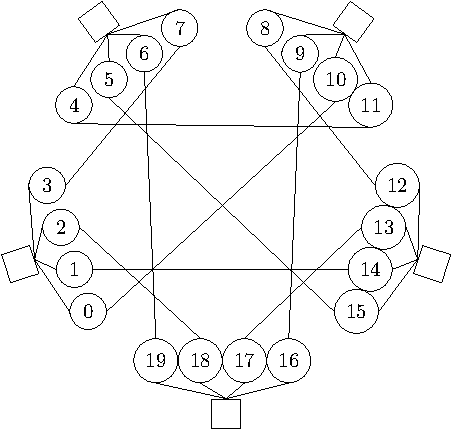
\includegraphics[width=1\textwidth]{figures/topologies/dcell-crop}
        \subcaption{Dcell$_1$ with 4 port switches \cite{GuoWTSZL08}}
    \end{minipage}\hfill
    \begin{minipage}{.53\textwidth}
        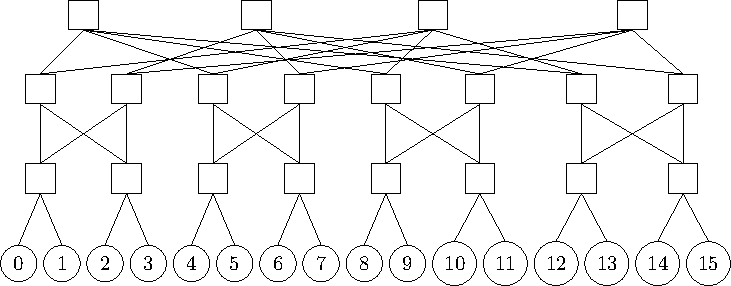
\includegraphics[width=\textwidth]{figures/topologies/fattree}
        \subcaption{Fat Tree with 4 port switches \cite{Al-FaresLV08}}

        \vspace{2.5em}

        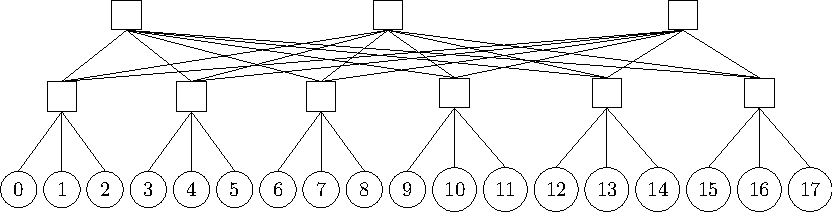
\includegraphics[width=\textwidth]{figures/topologies/leafspine}
        \subcaption{Leaf-Spine with 6 port switches \cite{Cisco19}}
    \end{minipage}\hfill
    \vspace{3em}
    \centering{
        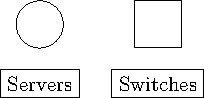
\includegraphics[width=0.2\textwidth]{figures/topologies/key}
    }
    \caption{Common datacenter topologies}
    \label{fig:topologies}
\end{figure*}

In this section, we describe the VNFPP and its constraints in detail. In the VNFPP, services must be placed on virtual machines in a datacenter so as to maximize multiple QoS objectives whilst minimizing energy consumption. The datacenter is a collection of servers interconnected by a network topology (see Fig. \ref{fig:topologies}). A service is a sequence of VNFs. Packets arrive at the first VNF in the service and must visit each VNF in sequence. A solution to the VNFPP places one or more instances of each VNF in the datacenter and specifies paths between VNFs to form services. 

The VNFPP has three objectives: two QoS metrics, latency and packet loss, and a cost metric, energy consumption. As service latency, packet loss and energy consumption conflict \cite{BillingsleyLMMG20} we formulate the VNFPP as a multi-objective optimization problem. Further, as services in a datacenter can number in the thousands it is not possible to treat each service quality metric as a separate objective. Instead, we aim to minimize the average service latency and the average service packet loss over all services, as well as the total energy consumption. Formally:

\begin{equation}
	\text{minimize} \ \textbf{F}\left(R_S\right) = \left(W, P, E\right)^T
	\label{eq:mo_formulation}
\end{equation}

\noindent where $R_S$ is the set of routes for each service, $W$ is the average service latency, $P$ is the average service packet loss and $E$ is the total electricity consumption of the datacenter. Several models exist to determine $W$, $P$ and $E$ for the VNFPP. This work uses the queueing theory model we proposed in \cite{BillingsleyLMMG19} and extended in \cite{BillingsleyJOURNAL}.

Finally, for a solution to the VNFPP to be feasible, it must satisfy two constraints. First, every VNF consumes some resources on a server. The total resources consumed by VNFs on a server cannot exceed the total resources of the server. Second, the solution must define one or more valid paths for each service. To be valid, a path must visit each VNF of the service in the order it appears in the service.


\section{Parallel MOEAs for the VNFPP}
\label{sec:algorithms}

In this section we outline the algorithms evaluated in this work and the genetic operators used to solve the VNFPP. First we describe the PMOEAs we evaluated and then we describe the genetic operators we have constructed to solve the VNFPP. 

\subsection{Parallel MOEA Frameworks}
PMOEAs can be grouped into three categories: master/slave algorithms, multiple-deme and isolated-deme algorithms \cite{Cantu-PazG99}. Each parallel algorithm distributes tasks over $N_T$ threads. In this work we evaluated a PMOEA from each category against a serial MOEA that does not use multithreading. The remainder of this section describes these algorithms in detail.

A serial MOEA is an evolutionary algorithm that only uses a single process. For this category, we selected the well known NSGA-II \cite{DebAPM00} algorithm, illustrated in Fig. \ref{fig:nsgaii}. NSGA-II maintains a population of $N$ parent solutions. A population of $N$ child solutions are generated via mutation and crossover of the parent population. Both populations are combined and then fast nondominated sorting and crowding distance procedures are used to determine which solutions survive to become the parent solutions of the next generation. This process repeats until the stopping condition is met. NSGA-II has been shown to be effective on a range of multiobjective optimization problems previously, including the VNFPP \cite{BillingsleyLMMG20}. Additionally, several parallel variants of NSGA-II exist, allowing for a fair comparison between single and multithreaded algorithms.

A master/slave algorithm has a single `master' thread that allocates tasks to `slave' threads. Once the slave threads are finished, the master thread aggregates the results. In this work we parallelise NSGA-II using this architecture, hereafter referred to as MS-NSGA-II (illustrated in Fig. \ref{fig:msnsgaii}). In this implementation each thread performs crossover, mutation and evaluation to produce $N / N_T$ solutions. Afterwards the solutions from each thread are aggregated to form the child population. As in NSGA-II, fast nondominated sorting and crowding distance procedures are used to select the parent population for the next generation. This process repeats until the stopping condition is met.

\begin{figure*}[t]
    \begin{minipage}{\textwidth}
        \centering
        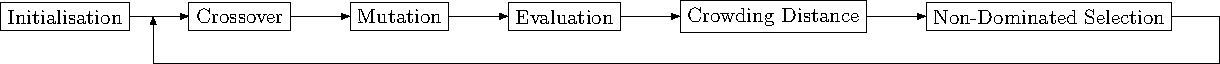
\includegraphics[width=\textwidth]{figures/algorithms/nsgaii}
        \subcaption{NSGA-II \cite{DebAPM00}}
        \label{fig:nsgaii}
    \end{minipage}
    \vspace{2.5em}

    \begin{minipage}{\textwidth}
        \centering
        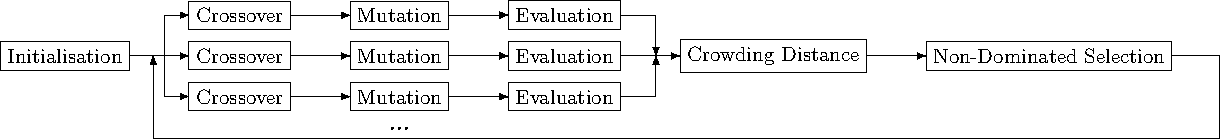
\includegraphics[width=\textwidth]{figures/algorithms/msnsgaii}
        \subcaption{MS-NSGA-II}
        \label{fig:msnsgaii}
    \end{minipage}
    \vspace{2.5em}

    \begin{minipage}{\textwidth}
        \centering
        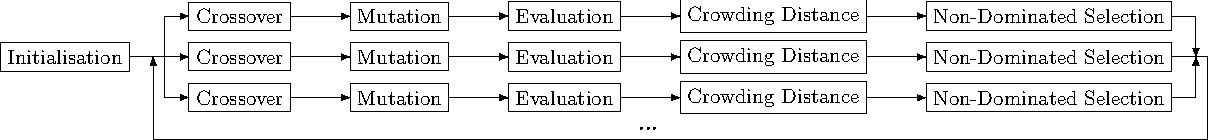
\includegraphics[width=\textwidth]{figures/algorithms/mdnsgaii}
        \subcaption{MD-NSGA-II \cite{RobergeTL13}}
        \label{fig:mdnsgaii}
    \end{minipage}
    \vspace{2.5em}

    \begin{minipage}{\textwidth}
        \centering
        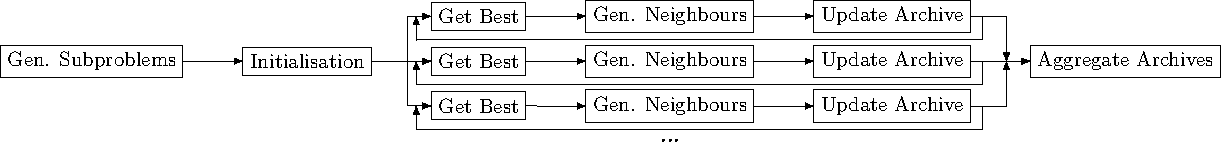
\includegraphics[width=\textwidth]{figures/algorithms/ppls}
        \subcaption{PPLS/D \cite{ShiZS20}}
        \label{fig:pplsd}
    \end{minipage}

    \vspace{1em}
    \caption{The four MOEAs we considered in this work. NSGA-II is a serial algorithm whilst the remaining parallelize some or all steps.}
    \label{fig:algorithms}
\end{figure*}

A multiple-deme algorithm evolves multiple subpopulations in parallel and periodically exchanges solutions between them. In this work we use the algorithm proposed by Roberge et al. \cite{RobergeTL13}, hereafter referred to as MD-NSGA-II, which uses a multiple-deme architecture (illustrated in Fig. \ref{fig:mdnsgaii}). Roberge et al. first produce a set of initial solutions and group them into $N_T$ equal sized subpopulations. The variation, evaluation and selection operators from NSGA-II are performed on each subpopulation in parallel. After a set number of generations, the subpopulations are aggregated into a new population and then randomly redistributed back into $N_T$ subpopulations. This process repeats until the stopping condition is met.

An isolated-deme algorithm also evolves multiple subpopulations but does not exchange information between the subpopulations. In this work we use the isolated-deme algorithm PPLS/D \cite{ShiZS20} (illustrated in Fig. \ref{fig:pplsd}). PPLS/D first decomposes the objective space into $N_T$ scalar objective optimization subproblems. The algorithm maintains a population of unexplored solutions and an archive of non-dominated solutions for each subproblem. First, a solution is added to the unexplored population of each subproblem. Next, for each subproblem the algorithm selects the best solution from the unexplored population and generates a set of neighboring solutions. A neighboring solution is added to the unexplored population and the non-dominated archive if it is: 1) closer to the subproblem that generated it than any other subproblem, as measured by the angle between the solution and the subproblems and 2) is either a better solution to the subproblem than the current best solution or if it is not dominated by any solutions in the non-dominated set of the subproblem. Once the stopping condition is met, the algorithm aggregates the non-dominated archives from each subproblem and returns the overall non-dominated solutions.

PPLS/D was designed for unconstrained optimization problems, so required modification to fit the VNFPP. In our variant, an infeasible solution is accepted into the unexplored population only if there are no more feasible solutions in the population. 

Additionally, to determine how PPLS/D is affected by the number of subproblems used, we generate $N$ subproblems that are placed into $N_T$ equally sized groups. Each subproblem in a group is executed in series and each group is executed in parallel. This technique produces solutions with the same solution quality as if greater numbers of threads were available whilst not unfairly benefitting PPLS/D.

\subsection{Genetic Operators}

\begin{figure}[t]
    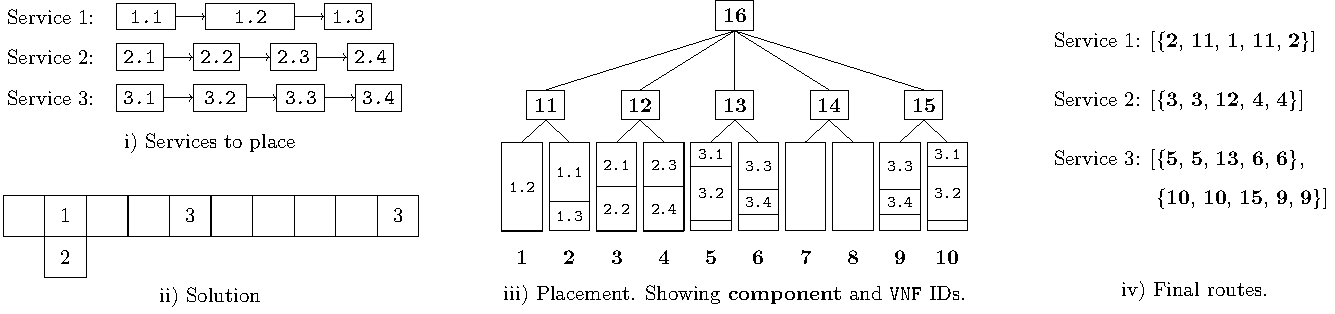
\includegraphics[width=\textwidth]{figures/algorithms/mapping}
    \caption{A partial mapping from genotype to phenotype showing the assignment of services to servers.}
    \label{fig:mapping}
\end{figure}

As this work focusses on the benefits of parallelisation, we use existing genetic operators that were designed for the VNFPP. In particular we use operators we demonstrated to be effective in earlier work \cite{BillingsleyLMMG20}. These operators use a genotype-phenotype representation where genetic operators consider a simplified solution representation (the genotype) which is converted into the `true' solution representation (the phenotype) to be evaluated. In our implementation, the genotype is an array of vectors where each vector represents a server in the datacenter (see Fig. \ref{fig:mapping} ii). Each vector contains zero or more service instances. The phenotype is the set of paths for each service (see Fig. \ref{fig:mapping} iv). The genotype-phenotype mapping has two parts: expansion and routing as shown in Fig. \ref{fig:mapping}. The expansion step iterates over each server in the genotype. When a service instance is encountered, the algorithm places each VNF of the service on the closest server that can accommodate it. The routing step finds the set of shortest paths between each VNF and combines them to form a path.

MD-NSGA-II and MS-NSGA-II require initialization, mutation, crossover and evaluation operators. PPLS/D additionally requires a local search operator. Since all services are considered equally important, the initialization operator always generates genotypes where each service has the same number of service instances. The operator first determines the maximum number of service instances that can be placed in a datacenter whilst meeting this constraint. Then it generates a range of solutions between the maximum and minimum number of service instances that can be placed. The mutation operator has an equal probability of 1) swapping the contents of two servers, 2) adding a random service instance to a random server and 3) removing a random service instance from a server. The same operator is used to generate neighbors in PPLS/D. Crossover is performed using the N-Point crossover.

\section{Experimental Results}
\label{sec:results}

In this section, we first describe our test methodology and then present the results. Our experiments were configured as follows. We generated 30 VNFPP instances for each problem size and topology by varying the number and length of services and the size and speed of the VNFs. We assigned each algorithm a budget of 16000 evaluations to be used across all threads. All tests were run on a 8 core/16 thread CPU at 2.6GHz. All parallel algorithms were implemented using the parallelisation library Rayon.\footnote[1]{\url{https://github.com/rayon-rs/rayon}}

We used the parameter settings for NSGA-II proposed in \cite{DebAPM00} for NSGA-II, MD-NSGA-II and MS-NSGA-II. As PPLS/D is known to be sensitive to the population size \cite{ShiZS20}, we also consider a range of population sizes for each test. 

For analysis, we recorded the time each algorithm took to complete and the hypervolume of the final population. Since the three objectives typically have orders of magnitude different values it is necessary to first normalize the objectives. The utopian and nadir points were estimated by taking the best and worst objective values respectively from all tests. We used the reference point $1 + \epsilon$ for each objective where $\epsilon$ is a small number.

\begin{figure}[t]
    \begin{minipage}{\textwidth}
        \hspace*{-2.1em}
        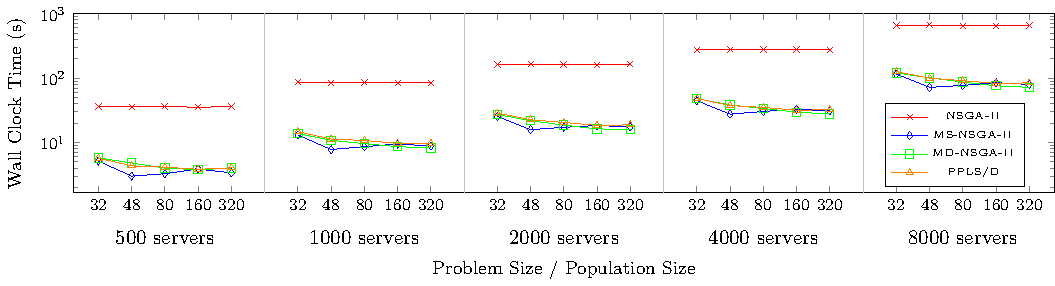
\includegraphics[width=1.05\textwidth]{figures/graphs/fat_tree_timing}
        \subcaption{Fat Tree}
        \vspace{1em}

        \label{fig:ft_tm}
    \end{minipage}

    \begin{minipage}{\textwidth}
        \hspace*{-2.1em}
        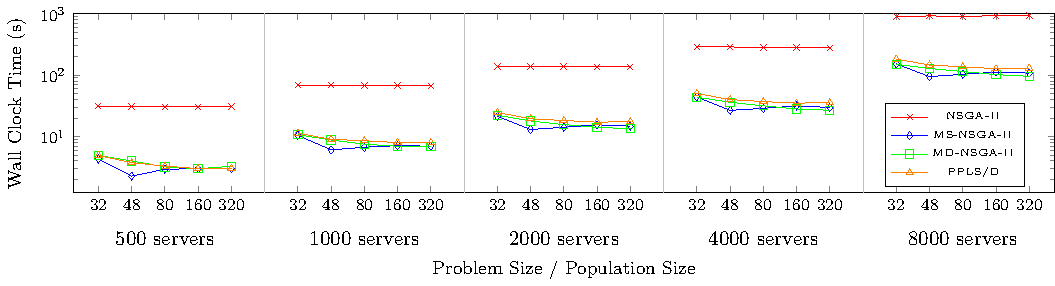
\includegraphics[width=1.05\textwidth]{figures/graphs/dcell_timing}
        \subcaption{DCell}
        \vspace{1em}

        \label{fig:dc_tm}
    \end{minipage}

    \begin{minipage}{\textwidth}
        \hspace*{-2.1em}
        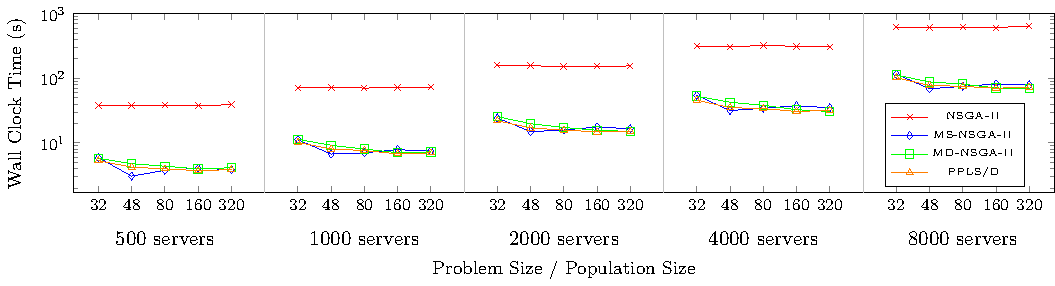
\includegraphics[width=1.05\textwidth]{figures/graphs/leaf_spine_timing}
        \subcaption{Leaf-Spine}
        \vspace{1em}

        \label{fig:ls_tm}
    \end{minipage}

    \caption{Mean Execution Time vs Problem Size and Population Size}
    \label{fig:et}
\end{figure}

\begin{figure}[t]
    \begin{minipage}{\textwidth}
        \hspace*{-2.1em}
        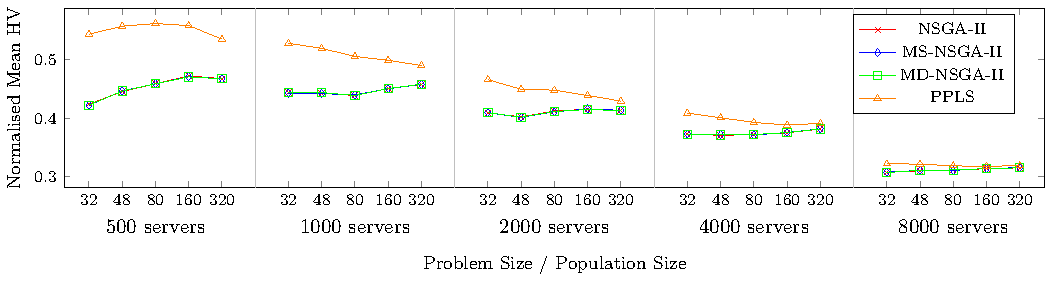
\includegraphics[width=1.05\textwidth]{figures/graphs/fat_tree_hv}
        \subcaption{Fat Tree}
        \vspace{1em}

        \label{fig:ft_hv}
    \end{minipage}

    \begin{minipage}{\textwidth}
        \hspace*{-2.1em}
        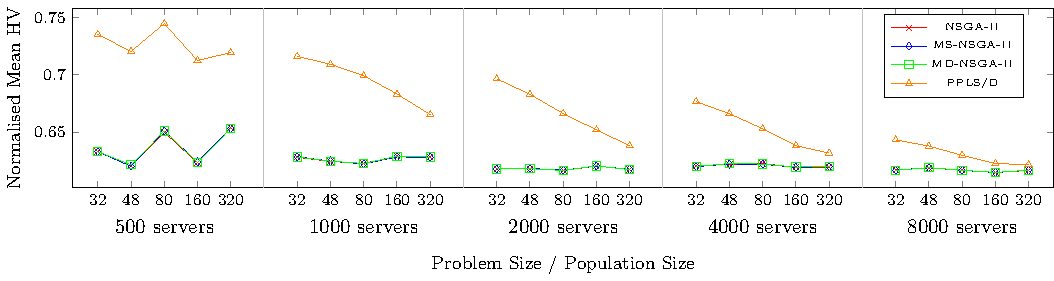
\includegraphics[width=1.05\textwidth]{figures/graphs/dcell_hv}
        \subcaption{DCell}
        \vspace{1em}

        \label{fig:dc_hv}
    \end{minipage}

    \begin{minipage}{\textwidth}
        \hspace*{-2.1em}
        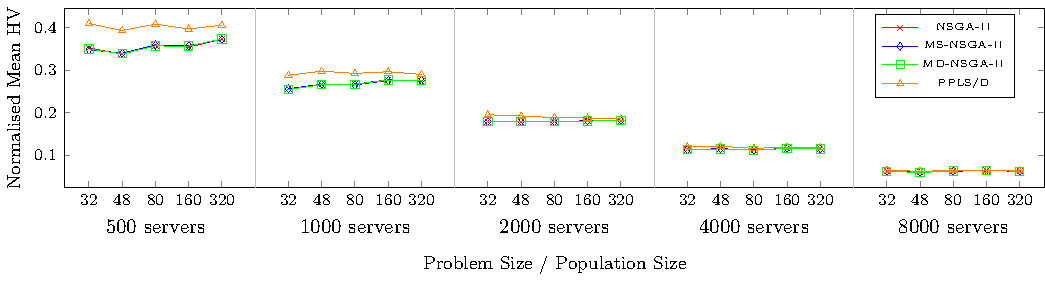
\includegraphics[width=1.05\textwidth]{figures/graphs/leaf_spine_hv}
        \subcaption{Leaf-Spine}
        \vspace{1em}

        \label{fig:ls_hv}
    \end{minipage}

    \caption{Mean HV vs Problem Size and Population Size}
    \label{fig:hv}
\end{figure}

Fig. \ref{fig:et} and Fig. \ref{fig:hv} demonstrate our two key findings. First, Fig. \ref{fig:et} shows that PMOEAs are typically 5-10x faster than the sequential NSGA-II. As the problem size increases, the time required to evaluate a solution also increases. However, this step can be parallelized reducing the overall execution time.

Second, Fig. \ref{fig:hv} shows that the speed improvements from parallelisation did not come at the cost of solution quality. This demonstrates that PMOEAs solve VNFPPs faster and at no cost to solution quality.

Further, when the best parameter settings are considered for each algorithm, PPLS/D found \textit{better} solutions on average than other algorithms on the majority of problems. These results must be considered with three caveats:

\begin{enumerate}
    \item PPLS/D was less effective on larger problem instances. Whilst all algorithms experienced some decline when solving larger problem instances, this behavior is particularly apparent with PPLS/D. PPLS/D relies on local search operators to explore the solution space. On large problem instances, the local search area is very large. It is likely that on large problems PPLS/D only explores the neighborhood of the initial population. Alternative local search operators may be able to explore the search space more effectively, however this remains for future research.

    \item PPLS/D is sensitive to the population size whereas the other algorithms were not. In the majority of instances, PPLS/D produced better sets of solutions when a small population was used. Shi et al \cite{ShiZS20} proposed this was due to large population sizes restricting each subproblem to a small region of the solution space. In PPLS/D, a subproblem can only consider a solution if it is the closest subproblem to the solution (see Section \ref{sec:algorithms}). With a large population, the solutions generated by the local search are more likely to be near to a different subproblem, reducing the number of solutions considered, and slowing the search process. This appears particularly important on larger problem instances wherein the setting of the population size was the most important factor in whether PPLS/D outperformed the other algorithms. 

    \item PPLS/D maintains an archive population and hence stores more solutions on the Pareto front than the other algorithms used. PPLS/D typically produced 1-2 orders of magnitude more non-dominated solutions than the other algorithms. This in part explains the improved hypervolume for PPLS/D as more solutions can better approximate the Pareto front.
\end{enumerate}

Despite these caveats, it is still notable that PPLS/D outperformed other algorithms using only local search operators. Some of the drawbacks of PPLS/D may be able to be resolved with alternative local search operators in future work.

\section{Conclusion}
\label{sec:conclusions}
In this work we determined whether PMOEAs could be used to solve the VNFPP more efficiently than sequential MOEAs without harming solution quality. We found that not only is this true, but that in certain instances PMOEAs produce better representations of the Pareto front than a comparable sequential algorithm. These results indicate that PMOEAs have potential to solve practical VNFPPs and are worthy of further research. Future work will explore alternative neighbor generation strategies to provide improved local search capabilities. Additional research could extend PMOEAs from single CPU, multithreaded systems to multi-cpu distributed systems in pursuit of larger speedups.

\bibliographystyle{splncs04}
\bibliography{bibliography}

\subsubsection*{Acknowledgements}
K. Li was supported by UKRI Future Leaders Fellowship (Grant No. MR/S017062/1) and Royal Society (Grant No. IEC/NSFC/170243). J. Billingsley was supported by EPSRC Industrial CASE and British Telecom (Grant No. 16000177). The authors would also like to acknowledge the use of the University of Exeter High-Performance Computing facility in carrying out this work and thank the developers and maintainers of Rust and the Rayon library.

\end{document}
